\PassOptionsToPackage{unicode=true}{hyperref} % options for packages loaded elsewhere
\PassOptionsToPackage{hyphens}{url}
%
\documentclass[]{article}
\usepackage{lmodern}
\usepackage{amssymb,amsmath}
\usepackage{ifxetex,ifluatex}
\usepackage{fixltx2e} % provides \textsubscript
\ifnum 0\ifxetex 1\fi\ifluatex 1\fi=0 % if pdftex
  \usepackage[T1]{fontenc}
  \usepackage[utf8]{inputenc}
  \usepackage{textcomp} % provides euro and other symbols
\else % if luatex or xelatex
  \usepackage{unicode-math}
  \defaultfontfeatures{Ligatures=TeX,Scale=MatchLowercase}
\fi
% use upquote if available, for straight quotes in verbatim environments
\IfFileExists{upquote.sty}{\usepackage{upquote}}{}
% use microtype if available
\IfFileExists{microtype.sty}{%
\usepackage[]{microtype}
\UseMicrotypeSet[protrusion]{basicmath} % disable protrusion for tt fonts
}{}
\IfFileExists{parskip.sty}{%
\usepackage{parskip}
}{% else
\setlength{\parindent}{0pt}
\setlength{\parskip}{6pt plus 2pt minus 1pt}
}
\usepackage{hyperref}
\hypersetup{
            pdftitle={Summer Research Project: Bats},
            pdfborder={0 0 0},
            breaklinks=true}
\urlstyle{same}  % don't use monospace font for urls
\usepackage[margin=1in]{geometry}
\usepackage{color}
\usepackage{fancyvrb}
\newcommand{\VerbBar}{|}
\newcommand{\VERB}{\Verb[commandchars=\\\{\}]}
\DefineVerbatimEnvironment{Highlighting}{Verbatim}{commandchars=\\\{\}}
% Add ',fontsize=\small' for more characters per line
\usepackage{framed}
\definecolor{shadecolor}{RGB}{248,248,248}
\newenvironment{Shaded}{\begin{snugshade}}{\end{snugshade}}
\newcommand{\AlertTok}[1]{\textcolor[rgb]{0.94,0.16,0.16}{#1}}
\newcommand{\AnnotationTok}[1]{\textcolor[rgb]{0.56,0.35,0.01}{\textbf{\textit{#1}}}}
\newcommand{\AttributeTok}[1]{\textcolor[rgb]{0.77,0.63,0.00}{#1}}
\newcommand{\BaseNTok}[1]{\textcolor[rgb]{0.00,0.00,0.81}{#1}}
\newcommand{\BuiltInTok}[1]{#1}
\newcommand{\CharTok}[1]{\textcolor[rgb]{0.31,0.60,0.02}{#1}}
\newcommand{\CommentTok}[1]{\textcolor[rgb]{0.56,0.35,0.01}{\textit{#1}}}
\newcommand{\CommentVarTok}[1]{\textcolor[rgb]{0.56,0.35,0.01}{\textbf{\textit{#1}}}}
\newcommand{\ConstantTok}[1]{\textcolor[rgb]{0.00,0.00,0.00}{#1}}
\newcommand{\ControlFlowTok}[1]{\textcolor[rgb]{0.13,0.29,0.53}{\textbf{#1}}}
\newcommand{\DataTypeTok}[1]{\textcolor[rgb]{0.13,0.29,0.53}{#1}}
\newcommand{\DecValTok}[1]{\textcolor[rgb]{0.00,0.00,0.81}{#1}}
\newcommand{\DocumentationTok}[1]{\textcolor[rgb]{0.56,0.35,0.01}{\textbf{\textit{#1}}}}
\newcommand{\ErrorTok}[1]{\textcolor[rgb]{0.64,0.00,0.00}{\textbf{#1}}}
\newcommand{\ExtensionTok}[1]{#1}
\newcommand{\FloatTok}[1]{\textcolor[rgb]{0.00,0.00,0.81}{#1}}
\newcommand{\FunctionTok}[1]{\textcolor[rgb]{0.00,0.00,0.00}{#1}}
\newcommand{\ImportTok}[1]{#1}
\newcommand{\InformationTok}[1]{\textcolor[rgb]{0.56,0.35,0.01}{\textbf{\textit{#1}}}}
\newcommand{\KeywordTok}[1]{\textcolor[rgb]{0.13,0.29,0.53}{\textbf{#1}}}
\newcommand{\NormalTok}[1]{#1}
\newcommand{\OperatorTok}[1]{\textcolor[rgb]{0.81,0.36,0.00}{\textbf{#1}}}
\newcommand{\OtherTok}[1]{\textcolor[rgb]{0.56,0.35,0.01}{#1}}
\newcommand{\PreprocessorTok}[1]{\textcolor[rgb]{0.56,0.35,0.01}{\textit{#1}}}
\newcommand{\RegionMarkerTok}[1]{#1}
\newcommand{\SpecialCharTok}[1]{\textcolor[rgb]{0.00,0.00,0.00}{#1}}
\newcommand{\SpecialStringTok}[1]{\textcolor[rgb]{0.31,0.60,0.02}{#1}}
\newcommand{\StringTok}[1]{\textcolor[rgb]{0.31,0.60,0.02}{#1}}
\newcommand{\VariableTok}[1]{\textcolor[rgb]{0.00,0.00,0.00}{#1}}
\newcommand{\VerbatimStringTok}[1]{\textcolor[rgb]{0.31,0.60,0.02}{#1}}
\newcommand{\WarningTok}[1]{\textcolor[rgb]{0.56,0.35,0.01}{\textbf{\textit{#1}}}}
\usepackage{graphicx,grffile}
\makeatletter
\def\maxwidth{\ifdim\Gin@nat@width>\linewidth\linewidth\else\Gin@nat@width\fi}
\def\maxheight{\ifdim\Gin@nat@height>\textheight\textheight\else\Gin@nat@height\fi}
\makeatother
% Scale images if necessary, so that they will not overflow the page
% margins by default, and it is still possible to overwrite the defaults
% using explicit options in \includegraphics[width, height, ...]{}
\setkeys{Gin}{width=\maxwidth,height=\maxheight,keepaspectratio}
\setlength{\emergencystretch}{3em}  % prevent overfull lines
\providecommand{\tightlist}{%
  \setlength{\itemsep}{0pt}\setlength{\parskip}{0pt}}
\setcounter{secnumdepth}{0}
% Redefines (sub)paragraphs to behave more like sections
\ifx\paragraph\undefined\else
\let\oldparagraph\paragraph
\renewcommand{\paragraph}[1]{\oldparagraph{#1}\mbox{}}
\fi
\ifx\subparagraph\undefined\else
\let\oldsubparagraph\subparagraph
\renewcommand{\subparagraph}[1]{\oldsubparagraph{#1}\mbox{}}
\fi

% set default figure placement to htbp
\makeatletter
\def\fps@figure{htbp}
\makeatother


\title{Summer Research Project: Bats}
\author{}
\date{\vspace{-2.5em}}

\begin{document}
\maketitle

\begin{center}\rule{0.5\linewidth}{0.5pt}\end{center}

\hypertarget{by-randy-posada}{%
\paragraph{\texorpdfstring{\emph{By Randy
Posada}}{By Randy Posada}}\label{by-randy-posada}}

\begin{center}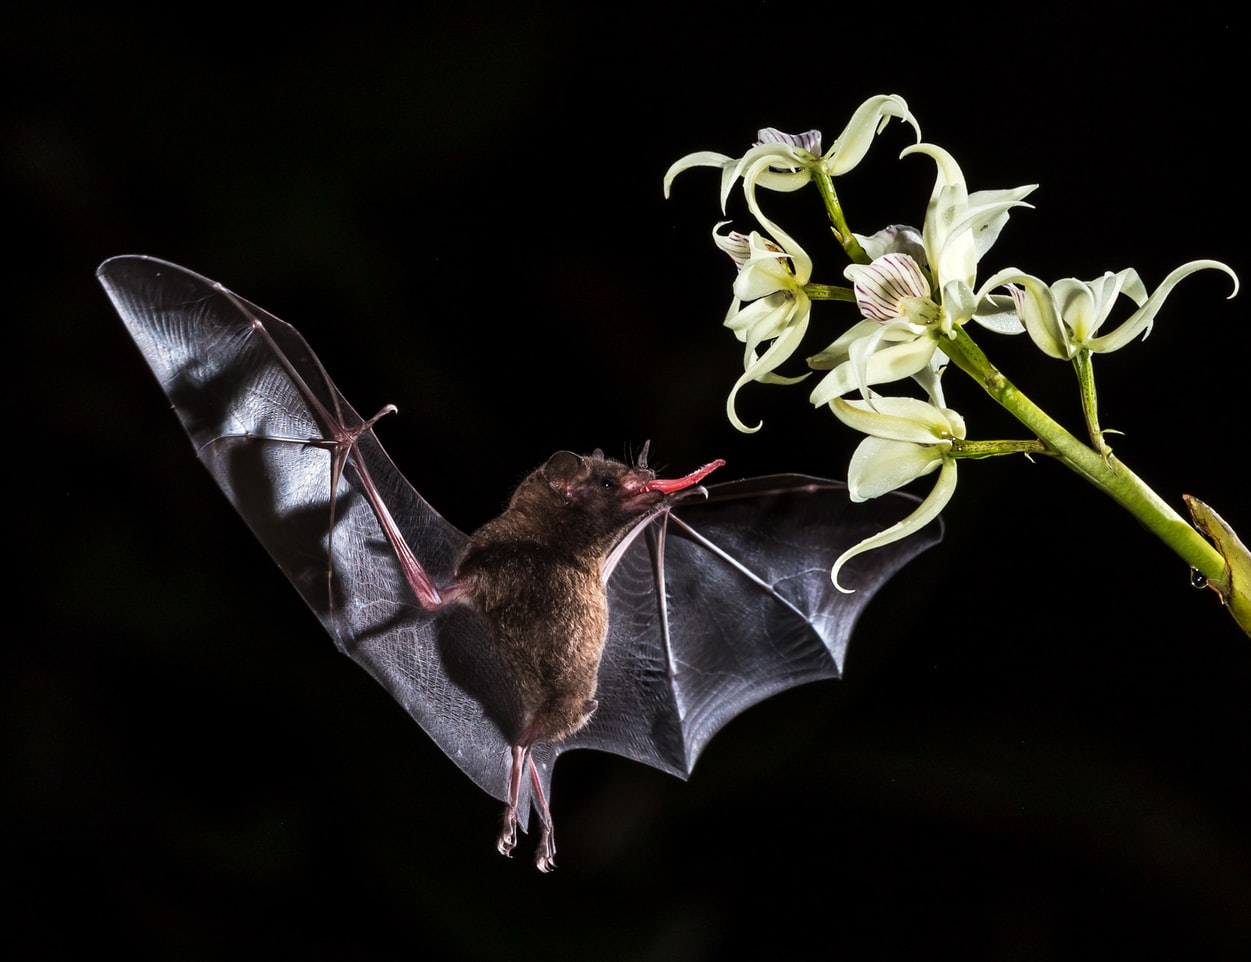
\includegraphics[width=1\linewidth,height=0.5\textheight]{../images/Batphoto1} \end{center}

\emph{Fig.cap="\protect\hyperlink{Attributions}{See attributions for
link}}

\begin{center}\rule{0.5\linewidth}{0.5pt}\end{center}

\hypertarget{my-report}{%
\section{\texorpdfstring{\textbf{My
Report}}{My Report}}\label{my-report}}

\hypertarget{overview}{%
\subsection{\texorpdfstring{\emph{Overview}}{Overview}}\label{overview}}

In this report I use the Open Tree of Life alongside Physcraper to
create and access an updated phylogentic tree of all bats.

There are over 1000 different species of bats. These extraordinary
flying mammals use their hands to fly; granted their order name
\emph{chiroptera}, which translates in Greek to `Hand Wings'. Each of
their fingers are connected to one another through a thin layer of skin
which allows these nocturnal mammals to take off into flight. Chiroptera
are the only mammals with the capability of continued flight.

\begin{center}\rule{0.5\linewidth}{0.5pt}\end{center}

\textbf{TASK 1: Add an intro to the Open Tree of Life.} \textbf{TASK 2:
How do we use tools from the Open Tree of Life with R? Talk about the
rotl package.}

\textbf{TASK 3: What does the tnrs\_match\_names function does?.}

\begin{Shaded}
\begin{Highlighting}[]

\NormalTok{my_taxa <-}\StringTok{ }\KeywordTok{c}\NormalTok{(}\StringTok{"chiroptera"}\NormalTok{)}
\NormalTok{resolved_names <-}\StringTok{ }\NormalTok{rotl}\OperatorTok{::}\KeywordTok{tnrs_match_names}\NormalTok{(}\DataTypeTok{names =}\NormalTok{ my_taxa)}

\NormalTok{resolved_names}
\CommentTok{#>   search_string unique_name approximate_match ott_id is_synonym flags}
\CommentTok{#> 1    chiroptera  Chiroptera             FALSE 574724      FALSE      }
\CommentTok{#>   number_matches}
\CommentTok{#> 1              1}
\end{Highlighting}
\end{Shaded}

It is useful to know the class of an object since it makes manipulating
objects much easier with different functions.When we create a class we
create a data structure that will house all the objects that belong to a
specific class. THis is done for ease of access, organization, and
clarity.

\begin{Shaded}
\begin{Highlighting}[]
\KeywordTok{class}\NormalTok{(resolved_names)}
\CommentTok{#> [1] "match_names" "data.frame"}
\end{Highlighting}
\end{Shaded}

The class of the resolved\_names object allows us to view the search
string name, the unique name ,and the ott\_id in respect to the open
tree of life. The class of the resolved\_names object which includes
`trns\_match\_names', allows us to view two outputs : ``match\_names''
and ``data\_frame''

In the following chunk, We can subset to obtain certain columns and and
if needed, manipulate the formula to extract a specific component from
the row. Since there is no function that allows us to extract the values
from a row of math\_names, we need to use resolved names and indexing.
Subsetting ultimately allows us to get values from all columns of one
row.

\begin{Shaded}
\begin{Highlighting}[]
\NormalTok{resolved_names[}\DecValTok{1}\NormalTok{,]}
\CommentTok{#>   search_string unique_name approximate_match ott_id is_synonym flags}
\CommentTok{#> 1    chiroptera  Chiroptera             FALSE 574724      FALSE      }
\CommentTok{#>   number_matches}
\CommentTok{#> 1              1}
\end{Highlighting}
\end{Shaded}

This is part of the previous chunk.

Our goal is to obtain the ott\_id for bats (Chiroptera). In order to
extract the information we need to subset using the column name
`unique\_name' in the second part of the formula `resolved\_names'. This
way, we can extract one specific value ( ) from the column we want using
the column name.

An OTT id is a unique numerical identifier assigned to a taxon in the
Open Tree Taxonomy. Every taxon has a specific OTT id. These OTT ids
allow us to interact with the Open Tree of Life.

If we want to obtain the unique name of the taxon used in the synthetic
open tree of life, we can use the following function. This function
takes into account our previous output of data and extract a specific
value.

\begin{Shaded}
\begin{Highlighting}[]
\NormalTok{resolved_names[}\DecValTok{1}\NormalTok{,}\StringTok{"unique_name"}\NormalTok{]}
\CommentTok{#> [1] "Chiroptera"}
\end{Highlighting}
\end{Shaded}

The next code gives all info from the current synthetic Open Tree:

\begin{Shaded}
\begin{Highlighting}[]
\NormalTok{rotl}\OperatorTok{::}\KeywordTok{tol_about}\NormalTok{()}
\CommentTok{#> }
\CommentTok{#> OpenTree Synthetic Tree of Life.}
\CommentTok{#> }
\CommentTok{#> Tree version: opentree12.3}
\CommentTok{#> Taxonomy version: 3.2draft9}
\CommentTok{#> Constructed on: 2019-12-23 11:41:23}
\CommentTok{#> Number of terminal taxa: 2391916}
\CommentTok{#> Number of source trees: 1216}
\CommentTok{#> Number of source studies: 1162}
\CommentTok{#> Source list present: false}
\CommentTok{#> Root taxon: cellular organisms}
\CommentTok{#> Root ott_id: 93302}
\CommentTok{#> Root node_id: ott93302}
\end{Highlighting}
\end{Shaded}

The previous code gave an output of the information from the Synthetic
Opent Tree of Life (OTOL) using the package `rotl'

This function assigns our matched name `chiroptera' to
``Chiroptera\_ott\_id'' and will therefore extract the ott\_id we wanted
for chiroptera once we run it.

\begin{Shaded}
\begin{Highlighting}[]
\NormalTok{chiroptera_ott_id <-}\StringTok{ }\NormalTok{rotl}\OperatorTok{::}\KeywordTok{tnrs_match_names}\NormalTok{(}\StringTok{"Chiroptera"}\NormalTok{)}\OperatorTok{$}\NormalTok{ott_id}
\NormalTok{chiroptera_ott_id}
\CommentTok{#> [1] 574724}
\end{Highlighting}
\end{Shaded}

The following code will help us get a subtree: \textbf{TASK 4: A subtree
of what?.}

\begin{Shaded}
\begin{Highlighting}[]
\NormalTok{chiroptera_subtree <-}\StringTok{ }\NormalTok{rotl}\OperatorTok{::}\KeywordTok{tol_subtree}\NormalTok{(}\DataTypeTok{ott_id =}\NormalTok{ chiroptera_ott_id)}

\NormalTok{ape}\OperatorTok{::}\KeywordTok{Ntip}\NormalTok{(chiroptera_subtree)}
\CommentTok{#> [1] 1820}

\NormalTok{ape}\OperatorTok{::}\KeywordTok{plot.phylo}\NormalTok{(chiroptera_subtree, }\DataTypeTok{cex =} \FloatTok{0.1}\NormalTok{, }\DataTypeTok{type =} \StringTok{"fan"}\NormalTok{)}
\end{Highlighting}
\end{Shaded}

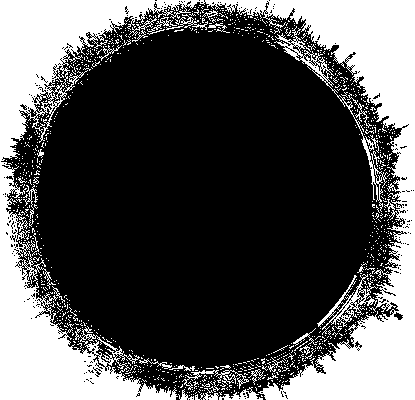
\includegraphics{report2_files/figure-latex/Obtaining_a_Subtree-1.pdf}

\begin{Shaded}
\begin{Highlighting}[]
\CommentTok{# or just plot(my_tree, cex = 0.1)}
\CommentTok{# because it has no branch lengths, it does not plot pretty. We have to get branch lengths for it.}
\CommentTok{# One way way to do this is to use datelife::datelife_search()}
\CommentTok{# Another way to do it is to make up teh branch lengths with ape::compute.brlen()}
\end{Highlighting}
\end{Shaded}

This will tell you if the taxon is monophyletic:

It is relevant that our taxon is monophyletic since nonmonophyletic taxa
contain `invalid' or `broken' data. When the taxon is `broken', its
ott\_id is not assidigned to a node in the synthetic tree.

\begin{Shaded}
\begin{Highlighting}[]
\NormalTok{rotl}\OperatorTok{::}\KeywordTok{is_in_tree}\NormalTok{(chiroptera_ott_id)}
\CommentTok{#> [1] TRUE}
\end{Highlighting}
\end{Shaded}

The above code confirmed that indeed our taxon is monophyletic by giving
the output `TRUE'

OTT ids and node ids allow us to interact with the synthetic OTOL.

\begin{Shaded}
\begin{Highlighting}[]
\NormalTok{chiroptera_node_info <-}\StringTok{ }\NormalTok{rotl}\OperatorTok{::}\KeywordTok{tol_node_info}\NormalTok{(chiroptera_ott_id)}
\NormalTok{chiroptera_node_info}
\CommentTok{#> }
\CommentTok{#> OpenTree node.}
\CommentTok{#> }
\CommentTok{#> Node id: ott574724}
\CommentTok{#> Number of terminal descendants: 1820}
\CommentTok{#> Is taxon: TRUE}
\CommentTok{#> Name: Chiroptera}
\CommentTok{#> Rank: order}
\CommentTok{#> ott id: 574724}
\end{Highlighting}
\end{Shaded}

We can use another R package --\texttt{datelife}, to get and plot a tree
of chiroptera families:

\begin{Shaded}
\begin{Highlighting}[]
\NormalTok{chiroptera_families <-}\StringTok{ }\NormalTok{datelife}\OperatorTok{::}\KeywordTok{get_ott_children}\NormalTok{(}\DataTypeTok{ott_ids =}\NormalTok{ chiroptera_ott_id, }\DataTypeTok{ott_rank =} \StringTok{"family"}\NormalTok{)}
\CommentTok{#>   |                                                                              |                                                                      |   0%  |                                                                              |======================================================================| 100%}
\CommentTok{#>   |                                                                              |                                                                      |   0%  |                                                                              |===================================                                   |  50%  |                                                                              |======================================================================| 100%}
\KeywordTok{ls}\NormalTok{(chiroptera_families)}
\CommentTok{#> [1] "Chiroptera"}
\NormalTok{chiroptera_families}
\CommentTok{#> $Chiroptera}
\CommentTok{#>                   ott_id   rank}
\CommentTok{#> Pteropodidae      574742 family}
\CommentTok{#> Myzopodidae         6788 family}
\CommentTok{#> Molossidae        238416 family}
\CommentTok{#> Vespertilionidae  238434 family}
\CommentTok{#> Thyropteridae     267980 family}
\CommentTok{#> Rhinopomatidae    267987 family}
\CommentTok{#> Hipposideridae    316928 family}
\CommentTok{#> Craseonycteridae   32051 family}
\CommentTok{#> Rhinolophidae     635025 family}
\CommentTok{#> Mystacinidae      759857 family}
\CommentTok{#> Noctilionidae     759861 family}
\CommentTok{#> Furipteridae     1060468 family}
\CommentTok{#> Emballonuridae    581454 family}
\CommentTok{#> Phyllostomidae    289151 family}
\CommentTok{#> Nycteridae       1018272 family}
\CommentTok{#> Natalidae        1018309 family}
\CommentTok{#> Mormoopidae       292475 family}
\CommentTok{#> Rhinonycteridae  5819794 family}
\CommentTok{#> Megadermatidae    813048 family}
\end{Highlighting}
\end{Shaded}

Using Chiroptera Families to create tree

\begin{Shaded}
\begin{Highlighting}[]
\NormalTok{chiroptera_families_subtree <-}\StringTok{ }\NormalTok{rotl}\OperatorTok{::}\KeywordTok{tol_induced_subtree}\NormalTok{(chiroptera_families}\OperatorTok{$}\NormalTok{Chiroptera}\OperatorTok{$}\NormalTok{ott_id)}
\CommentTok{#> Warning in collapse_singles(tr, show_progress): Dropping singleton nodes with}
\CommentTok{#> labels: Megachiroptera ott754606, mrcaott31957ott221782, mrcaott31957ott798260}
\end{Highlighting}
\end{Shaded}

Observing Tree Info

\begin{Shaded}
\begin{Highlighting}[]
\NormalTok{chiroptera_families_subtree}
\CommentTok{#> }
\CommentTok{#> Phylogenetic tree with 18 tips and 17 internal nodes.}
\CommentTok{#> }
\CommentTok{#> Tip labels:}
\CommentTok{#>  Vespertilionidae_ott238434, Molossidae_ott238416, Natalidae_ott1018309, Myzopodidae_ott6788, Phyllostomidae_ott289151, Mormoopidae_ott292475, ...}
\CommentTok{#> Node labels:}
\CommentTok{#>  Chiroptera ott574724, mrcaott6790ott6794, mrcaott6790ott6795, mrcaott6790ott130215, mrcaott6794ott73572, mrcaott6794ott9379, ...}
\CommentTok{#> }
\CommentTok{#> Rooted; no branch lengths.}
\end{Highlighting}
\end{Shaded}

Plotting Tree Of Chiroptera Families

\begin{Shaded}
\begin{Highlighting}[]
\NormalTok{ape}\OperatorTok{::}\KeywordTok{plot.phylo}\NormalTok{(chiroptera_families_subtree, }\DataTypeTok{cex =} \FloatTok{0.8}\NormalTok{)}
\end{Highlighting}
\end{Shaded}

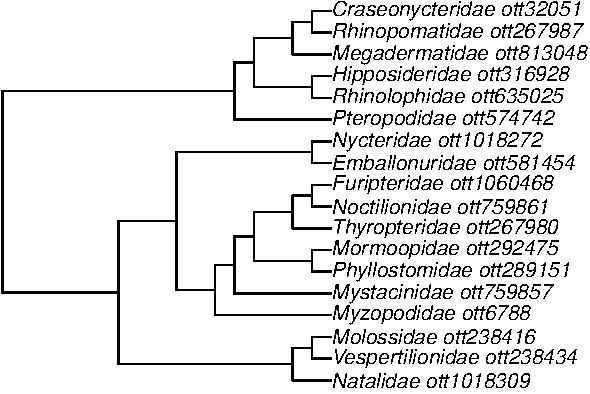
\includegraphics{report2_files/figure-latex/plot_subtree1-1.pdf}

Figure out how to get the ott ids as a vector.

\begin{Shaded}
\begin{Highlighting}[]
\NormalTok{chiroptera_families}\OperatorTok{$}\NormalTok{Chiroptera}\OperatorTok{$}\NormalTok{ott_id}
\CommentTok{#>  [1]  574742    6788  238416  238434  267980  267987  316928   32051  635025}
\CommentTok{#> [10]  759857  759861 1060468  581454  289151 1018272 1018309  292475 5819794}
\CommentTok{#> [19]  813048}
\end{Highlighting}
\end{Shaded}

\begin{Shaded}
\begin{Highlighting}[]
\KeywordTok{c}\NormalTok{(chiroptera_families}\OperatorTok{$}\NormalTok{Chiroptera}\OperatorTok{$}\NormalTok{ott_id)}
\CommentTok{#>  [1]  574742    6788  238416  238434  267980  267987  316928   32051  635025}
\CommentTok{#> [10]  759857  759861 1060468  581454  289151 1018272 1018309  292475 5819794}
\CommentTok{#> [19]  813048}
\end{Highlighting}
\end{Shaded}

To get an even smaller bat tree with 5 taxa that you like: First get the
scientific names of families, genera or species of bats. Then run
my\_ott\_ids \textless{}- rotl::tnrs\_match\_names to get the OTT ids

here I chose:
``Megadermatidae'',``Mormoopidae'',``Vespertilionidae'',``Mystacinidae'',and
``Furipteridae.''

\begin{Shaded}
\begin{Highlighting}[]
\NormalTok{my_ott_ids <-}\StringTok{ }\NormalTok{rotl}\OperatorTok{::}\KeywordTok{tnrs_match_names}\NormalTok{(}\KeywordTok{c}\NormalTok{(}\StringTok{"Megadermatidae"}\NormalTok{,}\StringTok{"Mormoopidae"}\NormalTok{,}\StringTok{"Vespertilionidae"}\NormalTok{,}\StringTok{"Mystacinidae"}\NormalTok{,}\StringTok{"Furipteridae"}\NormalTok{))}
\end{Highlighting}
\end{Shaded}

We will need to extract the ott ids only, because now we have the whole
table.

\begin{Shaded}
\begin{Highlighting}[]
\NormalTok{my_ott_ids}
\CommentTok{#>      search_string      unique_name approximate_match  ott_id is_synonym flags}
\CommentTok{#> 1   megadermatidae   Megadermatidae             FALSE  813048      FALSE      }
\CommentTok{#> 2      mormoopidae      Mormoopidae             FALSE  292475      FALSE      }
\CommentTok{#> 3 vespertilionidae Vespertilionidae             FALSE  238434      FALSE      }
\CommentTok{#> 4     mystacinidae     Mystacinidae             FALSE  759857      FALSE      }
\CommentTok{#> 5     furipteridae     Furipteridae             FALSE 1060468      FALSE      }
\CommentTok{#>   number_matches}
\CommentTok{#> 1              1}
\CommentTok{#> 2              1}
\CommentTok{#> 3              1}
\CommentTok{#> 4              1}
\CommentTok{#> 5              1}
\end{Highlighting}
\end{Shaded}

\begin{Shaded}
\begin{Highlighting}[]
\NormalTok{my_tree <-}\StringTok{ }\NormalTok{rotl}\OperatorTok{::}\KeywordTok{tol_induced_subtree}\NormalTok{(my_ott_ids}\OperatorTok{$}\NormalTok{ott_id)}
\CommentTok{#> Warning in collapse_singles(tr, show_progress): Dropping singleton nodes}
\CommentTok{#> with labels: mrcaott6790ott6795, mrcaott6790ott130215, mrcaott6794ott73572,}
\CommentTok{#> mrcaott6794ott9379, mrcaott9379ott167316, mrcaott263938ott604404,}
\CommentTok{#> mrcaott604404ott1060469, mrcaott10730ott31957, mrcaott31957ott79793,}
\CommentTok{#> mrcaott79793ott289141}
\end{Highlighting}
\end{Shaded}

This code chunk provides us with the info of our tree.

\begin{Shaded}
\begin{Highlighting}[]
\NormalTok{my_tree}
\CommentTok{#> }
\CommentTok{#> Phylogenetic tree with 5 tips and 4 internal nodes.}
\CommentTok{#> }
\CommentTok{#> Tip labels:}
\CommentTok{#> [1] "Vespertilionidae_ott238434" "Mormoopidae_ott292475"     }
\CommentTok{#> [3] "Furipteridae_ott1060468"    "Mystacinidae_ott759857"    }
\CommentTok{#> [5] "Megadermatidae_ott813048"  }
\CommentTok{#> Node labels:}
\CommentTok{#> [1] "Chiroptera ott574724" "mrcaott6790ott6794"   "mrcaott9379ott604409"}
\CommentTok{#> [4] "mrcaott9379ott263938"}
\CommentTok{#> }
\CommentTok{#> Rooted; no branch lengths.}
\end{Highlighting}
\end{Shaded}

To plot the above tree, the ape functiopn ``plot.phylo'' is used.

\begin{Shaded}
\begin{Highlighting}[]
\NormalTok{ape}\OperatorTok{::}\KeywordTok{plot.phylo}\NormalTok{(my_tree, }\DataTypeTok{cex =} \DecValTok{1}\NormalTok{)}
\end{Highlighting}
\end{Shaded}

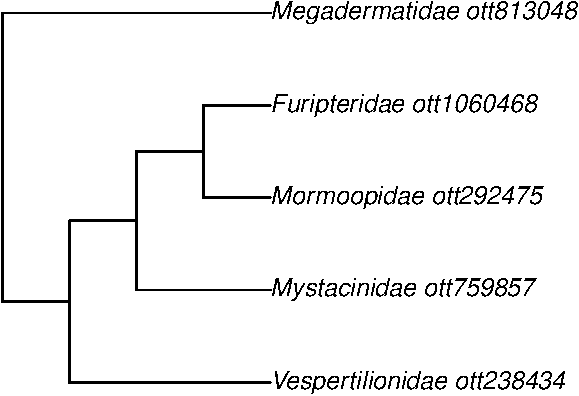
\includegraphics{report2_files/figure-latex/Plotting_my_tree-1.pdf}

\textbf{TASK 5: Describe how do you get help to use a function in R?}

\textbf{TASK 6: Run the datelife::get\_datelife\_result function for the
Chiroptera families.}

\begin{Shaded}
\begin{Highlighting}[]
\CommentTok{# YOUR_DATELIFE_RESULT_OBJECT <- datelife::get_datelife_result}
\end{Highlighting}
\end{Shaded}

\textbf{TASK 7: Take the output from datelife::get\_datelife\_result and
run the following code chunk.}

\begin{Shaded}
\begin{Highlighting}[]
 \CommentTok{# chiroptera_phylo_all <- datelife::summarize_datelife_result(YOUR_DATELIFE_RESULT_OBJECT, summary_format = "phylo_all")  (For Luna: What can i place as my datelife result object?)}

\CommentTok{# datelife::plot_phylo_all(trees = chiroptera_phylo_all)}
\end{Highlighting}
\end{Shaded}

\begin{center}\rule{0.5\linewidth}{0.5pt}\end{center}

\begin{Shaded}
\begin{Highlighting}[]
\NormalTok{chiroptera_node_subtree <-}\StringTok{ }\NormalTok{rotl}\OperatorTok{::}\KeywordTok{tol_subtree}\NormalTok{(}\DataTypeTok{node_id =}\NormalTok{ chiroptera_node_info}\OperatorTok{$}\NormalTok{node_id, }\DataTypeTok{label =} \StringTok{"name"}\NormalTok{)}
\CommentTok{#> Warning in collapse_singles(tr, show_progress): Dropping singleton nodes with}
\CommentTok{#> labels: Murina aurata, Murina huttoni, Eudiscopus, Myotis cf. nipalensis,}
\CommentTok{#> Myotis muricola, Myotis siligorensis, Myotis bombinus, Myotis myotis, Myotis}
\CommentTok{#> bocagii, Myotis nesopolus, Myotis oxyotus, Myotis martiniquensis, Myotis evotis,}
\CommentTok{#> Myotis brandtii, Submyotodon, Scotomanes, Ia, Lasionycteris, Nycticeinops,}
\CommentTok{#> Philetor, Pipistrellus javanicus, Nyctalus leisleri, Plecotus teneriffae,}
\CommentTok{#> Plecotus austriacus, Plecotus macrobullaris, Euderma, Idionycteris, Perimyotis,}
\CommentTok{#> Parastrellus, Lasiurus blossevillii, Dasypterus intermedius, Aeorestes}
\CommentTok{#> cinereus, Scotophilus viridis, Miniopterinae, Miniopterus griveaudi, Miniopterus}
\CommentTok{#> natalensis, Niumbaha, Scotozous, Scoteanax, Pharotis, Mimetillus, Atalapha,}
\CommentTok{#> Cynomops abrasus, Cynomops paranus, Eumops glaucinus, Eumops bonariensis,}
\CommentTok{#> Sauromys, Molossus currentium, Tomopeas, Platymops, Natalus stramineus,}
\CommentTok{#> Nyctiellus, Myzopodidae, Centurio senex, Sphaeronycteris, Pygoderma, Ametrida,}
\CommentTok{#> Ariteus, Ardops, Cubanycteris, Ectophylla, Platyrrhinus helleri, Platyrrhinus}
\CommentTok{#> lineatus, Mesophylla (genus in Opisthokonta), Sturnira lilium, Lionycteris,}
\CommentTok{#> Platalina, Xeronycteris, Lophostoma silvicolum, Macrophyllum, Vampyrum,}
\CommentTok{#> Chrotopterus, Brachyphyllinae, Brachyphylla nana, Lichonycteris, Musonycteris,}
\CommentTok{#> Choeronycteris, Hylonycteris, Diaemus, Neonycteris, Scleronycteris,}
\CommentTok{#> Dryadonycteris, Pteronotus davyi, Pteronotus personatus, Thyropteridae,}
\CommentTok{#> Noctilionidae, Amorphochilus, Mystacinidae, Emballonura semicaudata, Cormura,}
\CommentTok{#> Cyttarops, Mosia, Rhynchonycteris, Nycteridae, Megachiroptera, Boneia,}
\CommentTok{#> Mirimiri, Nyctimene albiventer, Pteropus pelewensis, Pteropus admiralitatum,}
\CommentTok{#> Pteropus rayneri, Pteropus samoensis, Pteropus anetianus, Pteropus capistratus,}
\CommentTok{#> Pteropus dasymallus, Pteropus melanotus, Melonycteris woodfordi, Nanonycteris,}
\CommentTok{#> Scotonycteris zenkeri, Chironax, Penthetor, Haplonycteris, Alionycteris,}
\CommentTok{#> Latidens, Sphaerias, Aproteles, Neopteryx, Plerotes, Hipposideros pomona,}
\CommentTok{#> Hipposideros ater, Hipposideros caffer, Hipposideros diadema, Anthops,}
\CommentTok{#> Macronycteris, Rhinonicteris, Cloeotis, Rhinolophidae, Rhinolophinae,}
\CommentTok{#> Rhinolophus lepidus, Rhinolophus rouxii, Rhinolophus sinicus, Rhinopomatidae,}
\CommentTok{#> Rhinopoma hardwickii, Craseonycteridae, Craseonycteris, Macroderma (genus in}
\CommentTok{#> Holozoa), Cardioderma, Lavia, Eudiscoderma, Archaeonycteridae, Icaronycteris,}
\CommentTok{#> Onychonycteridae, Onychonycteris}
\KeywordTok{head}\NormalTok{(chiroptera_node_subtree}\OperatorTok{$}\NormalTok{tip.label)}
\CommentTok{#> [1] "Kerivoula_hardwickii"  "Kerivoula_titania"     "Kerivoula_kachinensis"}
\CommentTok{#> [4] "Kerivoula_intermedia"  "Kerivoula_minuta"      "Kerivoula_whiteheadi"}
\end{Highlighting}
\end{Shaded}

\emph{Datelife Functions}

When you run the get datelife result function it will give node ages
from published trees that contain at least two taxa from your search:

\begin{Shaded}
\begin{Highlighting}[]
\NormalTok{chiroptera_dr <-}\StringTok{ }\NormalTok{datelife}\OperatorTok{::}\KeywordTok{get_datelife_result}\NormalTok{(chiroptera_node_subtree)}
\end{Highlighting}
\end{Shaded}

The datelife result object is not a tree but a list of tables with the
node ages for each pair of taxa from your search. For our 1800 species
in the Chiroptera, we got the following trees with node ages:

\begin{Shaded}
\begin{Highlighting}[]
\KeywordTok{names}\NormalTok{(chiroptera_dr)}
\CommentTok{#> [1] "Shi, Jeff J., Daniel L. Rabosky. 2015. Speciation dynamics during the global radiation of extant bats. Evolution 69 (6): 1528-1545"                                                                                                                            }
\CommentTok{#> [2] "Bininda-Emonds, Olaf R. P., Marcel Cardillo, Kate E. Jones, Ross D. E. MacPhee, Robin M. D. Beck, Richard Grenyer, Samantha A. Price, Rutger A. Vos, John L. Gittleman, Andy Purvis. 2007. The delayed rise of present-day mammals. Nature 446 (7135): 507-512"}
\CommentTok{#> [3] "Bininda-Emonds, Olaf R. P., Marcel Cardillo, Kate E. Jones, Ross D. E. MacPhee, Robin M. D. Beck, Richard Grenyer, Samantha A. Price, Rutger A. Vos, John L. Gittleman, Andy Purvis. 2007. The delayed rise of present-day mammals. Nature 446 (7135): 507-512"}
\CommentTok{#> [4] "Bininda-Emonds, Olaf R. P., Marcel Cardillo, Kate E. Jones, Ross D. E. MacPhee, Robin M. D. Beck, Richard Grenyer, Samantha A. Price, Rutger A. Vos, John L. Gittleman, Andy Purvis. 2007. The delayed rise of present-day mammals. Nature 446 (7135): 507-512"}
\CommentTok{#> [5] "Hedges, S. Blair, Julie Marin, Michael Suleski, Madeline Paymer, Sudhir Kumar. 2015. Tree of life reveals clock-like speciation and diversification. Molecular Biology and Evolution 32 (4): 835-845"                                                          }
\CommentTok{#> [6] "Lack J.B., & Van den bussche R.A. 2010. Identifying the Confounding Factors in Resolving Phylogenetic Relationships in Vespertilionidae. Journal of Mammalogy, ."                                                                                              }
\CommentTok{#> [7] "Dumont E.R., Davalos L.M., Goldberg A., Santana S.E., Rex K., & Voigt C.C. 2012. Morphological innovation, diversification and invasion of a new adaptive zone. Proceedings of the Royal Society B: Biological Sciences, 279: 1797-1805."}
\end{Highlighting}
\end{Shaded}

We have 7 studies in OpenTree with ages for the Chiroptera. The code
above provided all references of the seven studies as an output.

To get the actual chronograms we need to run another function:

\begin{Shaded}
\begin{Highlighting}[]
\NormalTok{chiroptera_phylo_all <-}\StringTok{  }\NormalTok{datelife}\OperatorTok{::}\KeywordTok{summarize_datelife_result}\NormalTok{(chiroptera_dr, }\DataTypeTok{summary_format =} \StringTok{"phylo_all"}\NormalTok{)}
\CommentTok{# We will write this object into a file, bc it takes a long time to run}
\KeywordTok{save}\NormalTok{(chiroptera_phylo_all, }\DataTypeTok{file=}\StringTok{"data/chiroptera_phylo_all.RData"}\NormalTok{)}
\end{Highlighting}
\end{Shaded}

Now, we have to load it into the R work space so it is available for the
next part

\begin{Shaded}
\begin{Highlighting}[]
\KeywordTok{load}\NormalTok{(}\StringTok{"../data/chiroptera_phylo_all.RData"}\NormalTok{)}
\end{Highlighting}
\end{Shaded}

The following function will allow us to plot the Tree with the ages.

\begin{Shaded}
\begin{Highlighting}[]
\NormalTok{datelife}\OperatorTok{::}\KeywordTok{plot_phylo_all}\NormalTok{(}\DataTypeTok{trees =}\NormalTok{ chiroptera_phylo_all, }\DataTypeTok{write=}\StringTok{"pdf"}\NormalTok{)}
\end{Highlighting}
\end{Shaded}

However, they are quite large, so we will not show them here for now.

Summarizing node ages is slow so we will save the output of
\texttt{datelife::summarize\_datelife\_result} in the data folder. This
function summarizes the node information from all the chronograms in
chiroptera\_phylo\_all.

\begin{Shaded}
\begin{Highlighting}[]
\NormalTok{chiroptera_phylo_median <-}\StringTok{  }\NormalTok{datelife}\OperatorTok{::}\KeywordTok{summarize_datelife_result}\NormalTok{(chiroptera_dr, }\DataTypeTok{summary_format =} \StringTok{"phylo_median"}\NormalTok{)}

\NormalTok{chiroptera_phylo_median}
\end{Highlighting}
\end{Shaded}

To plot the chronogram, Plotting Chronogram

\begin{Shaded}
\begin{Highlighting}[]
\NormalTok{ape}\OperatorTok{::}\KeywordTok{plot.phylo}\NormalTok{(chiroptera_phylo_median, }\DataTypeTok{cex =} \FloatTok{1.2}\NormalTok{)}
\CommentTok{# Add the time axis:}
\NormalTok{ape}\OperatorTok{::}\KeywordTok{axisPhylo}\NormalTok{()}
\CommentTok{# And a little hack to add the axis name:}
\NormalTok{graphics}\OperatorTok{::}\KeywordTok{mtext}\NormalTok{(}\StringTok{"Time (myrs)"}\NormalTok{, }\DataTypeTok{side =} \DecValTok{1}\NormalTok{, }\DataTypeTok{line =} \DecValTok{2}\NormalTok{, }\DataTypeTok{at =} \KeywordTok{max}\NormalTok{(}\KeywordTok{get}\NormalTok{(}\StringTok{"last_plot.phylo"}\NormalTok{,}\DataTypeTok{envir =}\NormalTok{ .PlotPhyloEnv)}\OperatorTok{$}\NormalTok{xx) }\OperatorTok{*}\StringTok{ }\FloatTok{0.5}\NormalTok{)}
\end{Highlighting}
\end{Shaded}

\hypertarget{running-python}{%
\section{running python}\label{running-python}}

** The \href{https://physcraper.readthedocs.io/en/latest/}{Physcraper}
software allow to update a published phylogeny with new DNA sequences
from \href{https://www.ncbi.nlm.nih.gov/genbank/}{GenBank.} This can be
your task for the fall if you are interested.**

\hypertarget{reproducibility}{%
\section{Reproducibility}\label{reproducibility}}

Do you want to reproduce this report yourself?

The following piece of code will render this report as pdf:

\hypertarget{attributions}{%
\section{Attributions}\label{attributions}}

\href{https://unsplash.com/photos/hNz4Qh9ECCc}{bat image}

\end{document}
